\documentclass[a4paper]{article}

\title{\vspace{-2.5em}\textsc{Machine Learning} Assignment 4 Report}
\author{\vspace{-.5em}110062219}
\date{}

\usepackage{amsmath}
\usepackage{amssymb}
\usepackage{caption}
\usepackage{float}
\usepackage{subcaption}
\usepackage{tikz}
\usepackage{pgfplots}
\usepackage{listings}
\usepackage[margin=2cm]{geometry}

\lstset{
	breaklines=true,
	basicstyle=\ttfamily,
}

\definecolor{nthu}{HTML}{7F1084}

% \renewcommand{\ttdefault}{pcr}

\begin{document}

\maketitle

\section{Problems Encountered}

In addition to the problems that have been discussed on eeclass, I stumbled on the problem that for sparse PCA, the given definition of \textit{sum of squared difference (SSD)} $\sum_{i=1}^N(\mathbf{x}_i-\mathbf{x_{proj}}_i)^2$ seemed awful since it's clear that $\mathbf{x}$, $\mathbf{x_{proj}}$ must have different shape --- the former would be $(n, 784)$ and the latter would be $(n, k)$. Other students and I coincidentally transformed $\mathbf{x_{proj}}$ back before computing \textit{SSD}. However, though we obtained results identical to expected output, it turned out that the convergence didn't achieved within 1000 iterations. So I would like to doubt whether they have any thing to do with?

Meanwhile, I also have reservations about the iterative method we're asked to realize sparse PCA. I lack confidence in the effect of only applying soft threshold and normalizing during each iteration. I would appreciate if you could provide some reference since I could hardly find any hint or clue.

\section{Implementation of Basic PCA}

First, the covariance matrix $\Sigma$ could be obtained by $\frac{1}{n}{X_{cent}}^TX_{cent}$. Then, we should compute the eigenvalues and eigenvectors to $\Sigma$, sort them in descending order of eigenvalues and cast them to real floats. Finally, we could pick first $k$ eigenvectors as our principal components.

\section{Eigenvectors and Reconstructed Image}

\begin{figure}[H]
\centering
\begin{subfigure}{.5\linewidth}
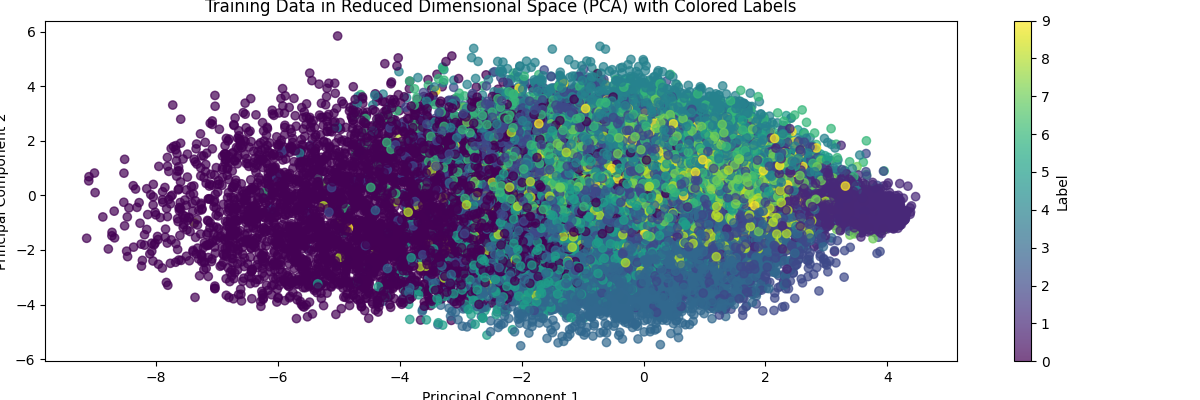
\includegraphics[width=\linewidth]{PCA_Training}
\caption{Eigenvectors}
\end{subfigure}
\begin{subfigure}{.3\linewidth}
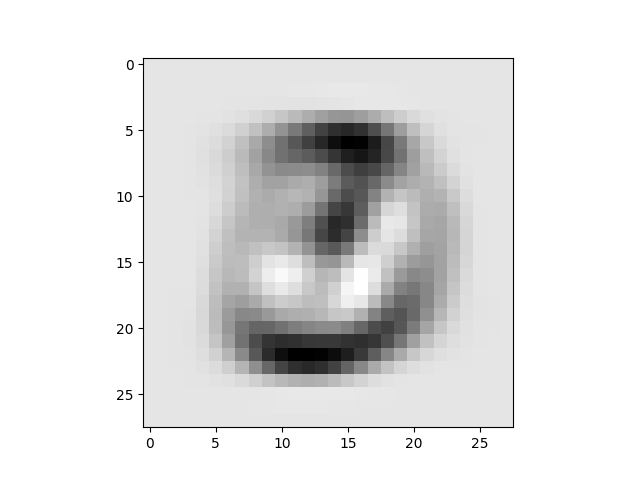
\includegraphics[width=\linewidth]{reconstruct_img}
\caption{Reconstructed Image}
\end{subfigure}
\caption{Eigenvectors and Reconstructed Image -- Training Data}
\end{figure}

\section{Distribution of Eigenvalues}

\begin{figure}[H]
\centering
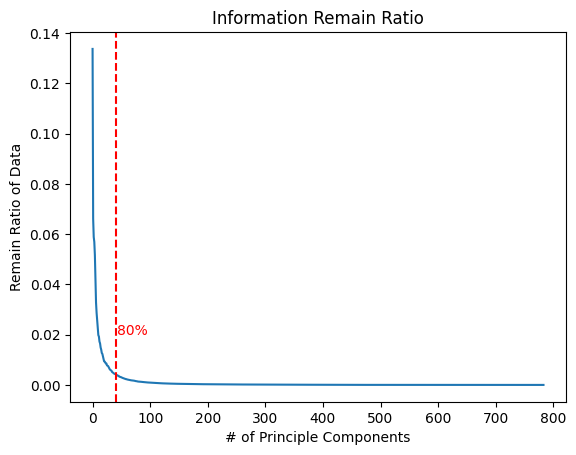
\includegraphics[width=.275\linewidth]{Infotmation Remaining Ratio}
\caption{Distribution of Eigenvalues}
\end{figure}

\section{Implementation of Advanced Part}

For advanced part, I normalized the data based on concatenation of training and testing data and randomly shuffled them. I adopted ordinary PCA and took $k=256$.

%\section*{Acknowledgements}
%
%I thank to \textsf{National Center for High-performance Computing} \textit{(NCHC)} for providing computational and storage resources.

\end{document}
